\chapter{A brief introduction to electric charges, currents, fields and potentials} 
\label{sec:Basics}
Action potentials are generated by electric currents over neural membranes. In turn, these currents
evoke the extracellular electric potentials that are the main topic of this book. 

Before we talk more about the electric signaling in the brain, we will in this chapter give a general introduction to the physics of electricity. The aim of this rather incomplete introduction is to establish an elementary understanding of the main concepts that we will use in the remainder of this book. Readers without prior schooling in physics will probably not be able to follow all parts of it, but it will hopefully still give them a basic understanding of the concepts of \textit{electric charge}, \textit{electic currents}, \textit{electric fields}, and \textit{electric potentials}, and some insight into how they are related to one another. Readers that do have a physics background might see it as a useful repetition. 

Most of the physics that we will go through is summarized in, and follows from, Maxwell's equations, and we might have kick-started this chapter by listing up those. However, since Maxwell's equations may appear a bit challenging for "the untrained eye", we will be taking a "softer" path, which we deem sufficient for establishing the main concepts that we will be working with. For good taste and later reference, we nevertheless go through Maxwell's equations in the final part of the chapter (Section \ref{sec:Basics:Maxwell}).


\section{\orange{GH: Electric charge}}
\label{Sec:Basics:Charge} \index{Charge}
Let us begin with the fundamental quantity for electricity, the electric charge. The fundamental charges are those carried by the protons and electrons that build up the atoms that build up the material world. The proton carries the \textit{unit charge} ($e$), while the electron has carries the negative unit charge $-e$, where $e = 1.602\times10^{-19}$ Coulomb (C). 

Since atoms contain an equal number of electrons and protons, most matter is electrically neutral. Some mediums are nevertheless conductive, which means that they contain so-called "free charge carriers", i.e., individual charges that may move through the medium. In an electric copper cable, such as that powering a lamp in a in a normal house, the free charge carriers are electrons that are not bound to specific locations (i.e., specific copper atoms), but can move freely through the copper material. In an electrolyte solution, for example salt-water, the free charge carriers are instead ions, i.e., atoms or molecules that have gained or donated one or several electrons, and therefore have become electrically charged. The saline solutions that fill the intracellular and extracellular space of the brain are such electrolytic solutions. Important charge carriers in the brain are sodium and potassium ions (Na$^+$ and K$^+$ with charge $1e$), chloride ions (Cl$^-$ with charge $-1e$, and calcium ions (Ca$^{2+}$ with charge $2e$).

At a fundamental, microscopic, level, electricity is largely due to the interactions between individual charges. A pair of charges, $q$ and $q'$, will act on each others with a force $F$, with units Newton (N) given by Coulomb's law:
\begin{equation}
F = k_e qq' \frac{1}{r^2}, 
\label{Basics:eq:CoulombF}
\end{equation}
where $k_e = 8.99\times10^9$ N$\cdot$ m$^2\cdot$C$^{-2}$ is Coulomb's constant, and $r$ is the distance between the two charges. The direction of the force is along the line between the two charges, and the force is inversely proportional to the square of the distance between them. The force will be repelling if the charges have the same valency (sign) and attractive if they have the opposite valency. 

We can express the direction of the force mathematically by use of a vector notation. Letting a boldface notation indicate that an entity is a vector, we may denote the positions of the charges $q$ and $q'$ by ${\bf r}$ and ${\bf r'}$, respectively. The position vector ${\bf r}$ can be visualized as an arrow from some reference point $r=0$ to the position of the charge $q$. Likewise, the vector ${\bf r}-{\bf r'}$ can be visualized from the position of $q'$ to the position of $q$, defining both the distance and direction of the (imagined) line connecting them. In vector notation, the force between the charge pair can be written:
\begin{equation}
{\bf F} = k_e q q' \frac{{\bf r}-{\bf r'}}{|{\bf r}-{\bf r'}|^3} = k_e  qq'  \frac{1}{|{\bf r}-{\bf r'}|^2} \frac{{\bf r}-{\bf r'}}{|{\bf r}-{\bf r'}|}.
\label{Basics:eq:CoulombFvec}
\end{equation}
Here, $|{\bf r}-{\bf r'}|$ denotes the length of the vector ${\bf r}-{\bf r'}$, i.e., the distance between the two charges, cf., $r$ in eq. \ref{Basics:eq:CoulombF}. In the rightmost expression, we have tried to illustrate the similarity to \ref{Basics:eq:CoulombF} expressing the splitting the magnitude and the direction of the force into two factors. The scalar factor $(k_e qq')/|{\bf r}-{\bf r'}|^2$ determines the force magnitude, and is the same as in eq. \ref{Basics:eq:CoulombF}. The remaining factor, $({\bf r}-{\bf r'})/|{\bf r}-{\bf r'}|$ is the division of a vector by its own length, and defines a \textit{unit vector}, a vector with length 1 defining the direction between the positions ${\bf r}$ and ${\bf r'}$, and thus of the force. 

If there are several point charges present, the contribution from each of them sum up linearly. If we have a charge $q$ in a position ${\bf r}$, the force acting on it by a number $N$ of other charges $q_1, q_2, q_3 ... q_N$ in positions ${\bf r_1}, {\bf r_2}, {\bf r_3} ... {\bf r_N}$ will then be:
\begin{equation}
{\bf F}({\bf r}) = \sum_{n=1}^N k_e q q_n \frac{{\bf r}-{\bf r_n}}{|{\bf r}-{\bf r_n}|^3}.
\label{Basics:eq:CoulombFN}
\end{equation}

If our system of study consisted of a small number $N_{small}$ of charges, we could use $N_{small}$ instances of eq. \ref{Basics:eq:CoulombFN} to compute the force acting on all the $N_{small}$ individual charges. Together with Newton's law ${\bf F} = m {\bf a}$, which tells us how the charges will be accelerated in the force direction, eq.\ref{Basics:eq:CoulombFN} would then allow us to compute the movements of all our charges over time. 

There is a fairly long way to go from eq. \ref{Basics:eq:CoulombF} to the understanding of electric phenomena in a macroscopic system such as for example the brain. When describing a macroscopic system, we are usually not interested in the microscopic interactions between a small number of charges, but rather the joint interactions of a very, very large number of charges. It is then not feasible to keep track of the motion of each individual charge. At the larger scale, we therefore do not want to work with forces acting on individual particles, but rather with the concept of electric fields, which we will define below. It is still nice to have taken a look at  Eq. \ref{Basics:eq:CoulombFN}, since it establishes the fundamental origin of electrical forces and fields. 


\section{\orange{GH: Electric fields}}
\label{sec:Basics:Fields} \index{Electric field}
The electric field at a given location (measured in volts per meter (V/m)) can be defined as the force that will act on a reference charge $q$ present there, i.e., 
\begin{equation}
{\bf E}({\bf r}) = {\bf F}({\bf r})/q.
\label{Basics:eq:E}
\end{equation}
If we assume that this force is exclusively due to the Coulomb interaction between electric charges, the electric field can be obtained by inserting eq. \ref{Basics:eq:CoulombFN} into eq. \ref{Basics:eq:E}:
\begin{equation}
{\bf E}({\bf r}) = \sum_{n=1}^N k_e q_n \frac{{\bf r}-{\bf r_n}}{|{\bf r}-{\bf r_n}|^3}.
\label{Basics:eq:CoulombEN}
\end{equation}

Like eq. \ref{Basics:eq:CoulombFN}, eq. \ref{Basics:eq:CoulombEN} applies to a microscopic level. For example, the field predicted by it will be big at locations that are close to an individual charge (i.e., at all locations where $|{\bf r}-{\bf r_n}|$ is small), and smaller at points where the distance to the nearest charge is longer. Since the average distance between ions in the saline solution of the brain is on the order of a nanometer, this means that the field will vary with a sub-nanometer resolution. A direct use of eq. \ref{Basics:eq:CoulombEN} will therefore, again, force us to keep track of each individual charge, which would not be feasible in a macroscopic system.

Fortunately, we do not have to care too much about these microscopic field variations when we are trying to understand the brain. A technical argument for why this is not the case, is that the electrodes used to record brain signals have a tip diameter which is typically a micrometer or more. This is much, much larger than the average intra-charge distance in the saline solution of the brain. The electrodes therefore do not "see" the microscopic fluctuations, but rather sense the average field taken over the electrode surface. When we speak of an electric field or electric potential in the brain, we therefore always mean field or potential on a so-called \textit{coarse-grained} scale, averaged over an electrode surface of at least $1 \mu$m$^2$. A non-technical argument is that it is this coarse-grained signal, and not the microscopic reality that is bubbling underneath it, that is of importance if we want to understand the key brain processes. 

From here on, we shall not think of ${\bf E}$ as something that we compute based on
knowledge of the microscopic charge distribution (cf. eg. \ref{Basics:eq:CoulombEN}), but rather as a higher level entity, exerting an average force on all charges in a certain direction.


\section{\orange{GH: Electric potentials}}
\label{sec:Basics:Potential} \index{Electric potential}
Tightly related to the electric field ${\bf E}$ is the electric potential $\phi$ (with units volt (V)), which is what we normally measure experimentally when we stick an electrode into the brain. While ${\bf E}$ is a fundamental physical entity, $\phi$ may be regarded as an auxiliary variable. It is a way to represent the electric field that often makes computations simpler and measurements easier. 

The electric field can be expressed as the spatial derivative, or gradient, of the potential:
\begin{equation}
{\bf E}(x,y,z) = - \nabla \phi(x,y,z) = - \left(\frac{d\phi}{dx} {\bf e_x}  + \frac{d\phi}{dy} {\bf e_y} + \frac{d\phi}{dz} {\bf e_z} \right) \phi.
\label{Basics:eq:EV}
\end{equation}
The operator $\nabla$ computes a property's spatial rate of change in the various spatial directions, and ${\bf e_x}$, ${\bf e_y}$ and  ${\bf e_z}$ are the unit vectors in the three spatial directions $x$, $y$ and $z$, respectively. Unlike ${\bf E}$, which is a vector-field, $\phi$ is a scalar function, and as such, it tends to be easier to deal with. We note that eq. \ref{Basics:eq:EV} rests on something called the \textit{quasi-static approximation} of Maxwell's equations, which we explain further in Section \label{sec:Basics:Maxwell}. 

To get an intuitive understanding of the relationship between ${\bf E}$ and $\phi$, it helps to consider an idealized one-dimensional scenario with a constant field in the $x$-direction. Then, eq. \ref{Basics:eq:EV} simplifies to,
\begin{equation}
E = -\frac{d\phi(x)}{dx} = -\frac{\Delta \phi}{\Delta x} = -\frac{\phi(x_b)-\phi(x_a)}{x_b-x_a},
\label{Basics:eq:EV1D}
\end{equation}
where the first equality follows from the 1D-assumption, the second from the assumption that $E$ is constant, and the third is simply a definition of the second, where $x_b$ and $x_a$ may represent any two arbitrary points in space. For example, if $E = 1$ V/m, and if the distance between our points $x_b-x_a$ is 1m, Eq. \ref{Basics:eq:EV1D} tells us that $\phi$ will be 1 V  lower in $x_b$ compared to $x_a$ (Fig. \ref{Basics:fig:Ground}).

\begin{figure}[!ht]
\begin{center}
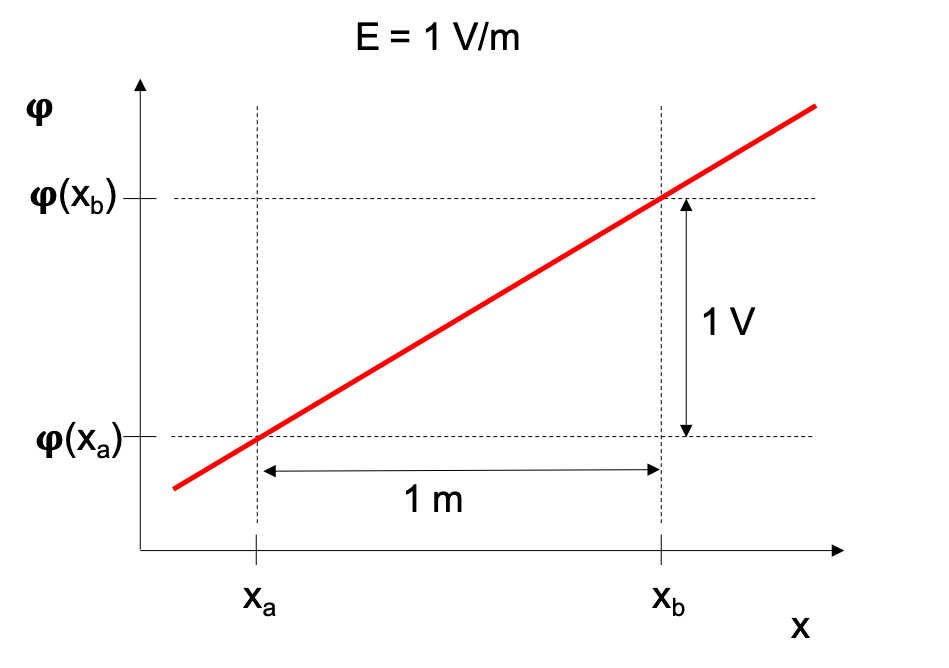
\includegraphics[width=0.8\textwidth]{Figures/Basics/Ground.png}
\end{center}
\caption{\textbf{Relationship between the electric field and electric potential.} With a constant electric field $E = 1$ V/m, the electric potential $\phi$ increases linearly with distance $x$. With two locations $x_a$ and $x_b$ 1 m apart, we know that $\phi(x_b) = \phi(x_a) + 1$ V. We are free to define an arbitrary reference point (ground) for the $\phi$, and if we take $\phi(x_a) = 0$, it follows that $\phi(x) = (x-x_a) \times E$. In $x_b$, we then get $\phi(x_b)=$(1m)$\times$1V/m$=1$ V. Equivalently, we might define $x_b$ as our reference point, which would mean that $\phi(x_b) = 0$ and $\phi(x_a) = -1$ V. Regardless of where we place our reference point, the physics (i.e., the field, $E$) would be the same.
}
\label{Basics:fig:Ground}
\end{figure}

We may use the example in Fig. \ref{Basics:fig:Ground} to define the important concept of \textit{ground}. The field ${\bf E}$ generally determines the potential only up to a constant. In the example, the field $E = 1$ V/m would be consistent with any pair of potentials $\phi_a$ and $\phi_b$ as long as $\phi_b - \phi_a =  1$ V. Since it is the field, and not the potential, that is the fundamental physical entity, we can therefore not speak of the potential in a certain point as an absolute entity, but only the potential \textit{difference} between two points. When we record potential in a given location, we must always record it relative to some an arbitrary reference point, which we call \textit{ground}, and where we define $\phi = 0$ (cf. example in Fig. \ref{Basics:fig:Ground}). 

When we record extracellular potentials, we can chose to place the reference electrode either outside or inside brain tissue \cite{Sharott2015}, but we typically want to keep it at some distance from the recording electrode, so that reference electrode is not affected by the processes that we investigate with the recording electrode. 

By definition, the electric potential is the energy needed to move a unit of electric charge $q$ from the reference point (ground) to a specific location in the electric field. The unit (V) of the electric potential is equivalent to energy per charge, or Joule per Coulomb (V = J/C). As such, the concept of an electric potential is closely related to the concept of a potential energy. The potential energy ($U_E$) of a charge $q$ in an electric field is:
\begin{equation}
U_E = q\phi.
\label{Basics:eq:UE}
\end{equation}


\section{\orange{GH: Electric current}}
\label{sec:Basics:Current} \index{Electric current}
As we have emphasized several times, we do not want to study the brain by keeping track of individual charges. We are rather interested in the net movement of charge at a coarse-grained (space averaged) scale. In an electrical copper cable, the movement of charge is normally described in terms of a electrical current $I$, which represents the total current through the cable as a whole, and has units Ampere (A = C/s). For currents in a three dimensional volume, such as brain tissue, it is more convenient to work with current densities, ${\bf i}$  which is defined as the current per unit cross section area, and has units A/(m$^2$).

Before defining the current density further, we need to say some words about the medium that it runs through. A bit simplistically, we may think of the brain as consisting of the intracellular saline solution, the extracellular saline solution, and the neuronal and glial membranes separating the two. Neural and glial membranes are largely dielectric (insulating) \index{Dielectricum} in their nature. In a dielectric medium, charges are bound to stay in confined regions of space, and an electric field only will slightly shift their average equilibrium positions, causing a polarization of the material. It is such a polarization that gives rise to the neuronal and glial membrane potentials. 

Unlike the dielectric membrane, the saline solutions that fill up the intra- and extracellular spaces are predominantly of conductive nature \index{Conductor}, which means that charges move rather freely through them when exposed to an electric field. As currents that pass through brain tissue predominantly move through the extracellular part of it, we shall represent the tissue as a conductor. 

For most parts of this book, we shall approximate brain tissue as a \textit{linear} conductor, which means that the tissue current densities are given by the formula:
\begin{equation}
{\bf i_t} = \sigma_t {\bf E},
\label{Basics:eq:i}
\end{equation}
where the index $t$ stands for tissue. Eq. \ref{Basics:eq:i} is a version of Ohm's law. It states that the current density will be proportional to the electric field and the conductivity of the medium, $\sigma_t$, which has units Siemens per square meters (S/m$^2$). The conductivity is a material property, and in brain tissue, it is often assumed to be a constant, at least within a given brain region. 

It is important to remember that the current given by eq. \ref{Basics:eq:i} represents the average movement of charge on a coarse-grained level, and does not apply on a microscopic scale. If we compare it with the microscopic fundament for this movement, it is easy to get confused, so let us dive into that confusion and try to clear it up. According to eq. \ref{Basics:eq:E}, an electric field will act on a reference charge $q$ by a constant force, which according to Newton's law (${\bf F} = m{\bf a}$) should give it a constant acceleration in the field-direction. Conversely, eq. \ref{Basics:eq:i} states that ${\bf E}$ gives rise not to a constant acceleration of charges, but rather a constant current, i.e., a constant average \textit{velocity} of charges. 

The reason for the discrepancy between the microscopic (constant acceleration) and macroscopic (constant velocity) level is that the constant acceleration (eq. \ref{Basics:eq:E}) at the microscopic level will go on for only a tiny time period (called the charge relaxation-time) \index{Charge-relaxation} before our protagonist charge $q$ will bump into some other particle and be scattered out in some random direction. After the scattering event, the acceleration will start "from scratch" again, and go on until the next collision takes place, and so forth. Whereas the scattering events will tend to make the motion of $q$ a random walk (which should give it a zero average velocity in any preferred direction), the small periods of acceleration between collisions will at average give $q$ a net drift velocity in the field direction. As the same will happen for all other charges present, there will be a net drift of charge in the field direction. The current density given by Eq. \ref{Basics:eq:i}, is therefore often referred to as the drift current density. Admittedly, the explanation that we proposed here was somewhat hand-waving, and the fact that we get the linear (constant velocity) relationship in eq. \ref{Basics:eq:i} is constitutive, meaning that it is observed experimentally rather than derived from first physical principles, and is found to be a good approximation for many mediums, brain tissue included, under many conditions \cite{Nunez2006,Pettersen2012}. 


\section{\orange{GH: Electroneutrality of brain tissue}}
\label{sec:Basics:Electroneutrality}
Due to the Coulomb force (eq. \ref{Basics:eq:CoulombF}), positive charges will repel other positive charges, and attract negative charges. An effect of this is that positive charges will tend to surround themselves with negative charges, and vice versa. Consequently, the numbers of positive and negative charges in a finite volume of space tends to be in balance, and any finite reference volume of brain tissue will, on the coarse-grained scale, be practically electroneutral \cite{Nunez2006,Grodzinsky2011}. If this were not the case, and a volume did contain a net charge density $\rho$, the very strong Coulomb-forces associated with it would cause $\rho$ to decay to zero at a rate proportional to the so-called \textit{charge-relaxation time}, which in brain tissue is in the order of a nanosecond \cite{Grodzinsky2011}. 

The Coulomb force also gives rise to a phenomenon called Debye shielding \cite{Nunez2006}. As positive charges will tend to surround themselves with negative charges, and vice versa, they will tend to shield (cancel out) the electric fields from one another, so that neither of them give any contribution to the field measured at some distance away from the charges.

Of course, a non-zero electric field or potential does require some charge separation somewhere. In the brain, this predominantly happens at neuronal membranes, and then on a very small spatial scale. Working as a parallel plate capacitor, a patch of membrane separates a charge $Q$ on the interior side from a charge $-Q$ on the exterior side. These two charges are equal in magnitude and opposite in sign, and are distributed in nanometer-thick sheaths on the interior and exterior membrane, called Debye layers. This charge separation gives rise to the membrane potential $V_m = Q/C_m$, where $C_m$ is the capacitance (with units Fahrad (F)) of the patch of membrane. We will speak more of the membrane capacitance in Chapter \ref{sec:Neuron}, but the point that we wanted to make here is that, since the membrane is just some nanometers thick, the two charges $-Q$ and $Q$ are very close in space, and will shield each others' contributions to extracellular fields measured at some distance from the membrane. 


\section{\orange{GH: Neurons as current sources}}
\label{sec:Basics:C} 
\index{Current source density}
The practical implication of electroneutrality and shielding effects is that, when we study extracellular potentials (or fields), we can neglect contributions from any particular distribution of charges, and instead compute extracellular potentials from the constraint that there should be no charge accumulation anywhere in the extracellular space. 

As we shall explain further in Chapter \ref{sec:VC}, the sources for the extracellular potential (of field) will then exclusively be the electric \textit{currents} entering or leaving the extracellular space through neural membranes. Mathematically, we can express this through the continuity equation:
\begin{equation}
\nabla \cdot {\bf i_t} = -C.
\label{Basics:eq:continuity1}
\end{equation}
where the source term, $C$, is called the current source density (units A/m$^3$), and represents  
the transmembrane output currents from neurons per tissue volume. We recall that ${\bf i_t}$ here is the density of current running extracellularly through brain tissue. It does not include intracellular or transmembrane neural currents. 

Eq. \ref{Basics:eq:continuity1} tells us that in a volume of space where there is no neuronal membrane ($C = 0$), we have that $\nabla \cdot {\bf i_t} = 0$. This means that there will be no net current entering or leaving such a volume. Importantly, this does not mean that the current must be zero. Currents can and will still run \textit{through} the volume.

In a volume that \textit{does} receive a neuronal output, eq. \ref{Basics:eq:continuity1} tells us that the current outputted from the neuron into that volume ($C$) must be carried away from that volume in terms of an extracellular tissue current. As we shall show in Chapter \ref{sec:VC}, this conservation law shall be the fundament for modeling extracellular potentials surrounding active neurons.


\section{\orange{GH: Maxwell's equations}}
\label{sec:Basics:Maxwell} \index{Maxwell's equations}
Most of the physics that we have gone through so far follows from Maxwell's equations, so we will summarize this chapter by going briefly through these. The equations come in two versions, referred to as the microscopic and macroscopic versions. The microscopic version is the most fundamental, but using it requires knowledge of the positions of all individual charges, which is unfeasible when any medium at a macroscopic level. We therefore only list up the macroscopic set of equations: 

\begin{eqnarray}
\nabla\cdot {\bf D} & = & \rho. \label{Basics:eq:Max1} \\
\nabla \cdot {\bf B} & = & 0.  \label{Basics:eq:Max2} \\
\nabla \times {\bf E} & = & - \frac{\partial {\bf B}}{\partial t}.  \label{Basics:eq:Max3} \\
\nabla \times {\bf H} & = & \bf{i} + \frac{\partial {\bf D}}{\partial t}.  \label{Basics:eq:Max4}
\label{Basics:eq:Maxwell}
\end{eqnarray}

Eq. \ref{Basics:eq:Max1} is called Gauss's law (for electricity). The variable ${\bf D}$ is called the \textit{displacement field}, and $\rho$ is the free (unbound) charge density, which generally can be non-zero, although we argued earlier that brain tissue for practical purposes can be assumed to be electroneutral at the coarse-grained scale. ${\bf D}$ is tightly related to the total electric field ${\bf E}$ that we have introduced earlier. In a linear dielectric medium (and we will in this book assume that our mediums are linear), it holds that ${\bf D} = \epsilon {\bf E}$, where $\epsilon$ is the electric permittivity of the medium. 

Eq. \ref{Basics:eq:Max2} is Gauss's law for magnetism, and is the magnetic equivalent to eq. \ref{Basics:eq:Max1}, with {\bf B} being the magnetic induction field.  Whereas eq. \ref{Basics:eq:Max1} states that there can be a spatial gradient of the electric field due to a local charge density $\rho$, eq. \ref{Basics:eq:Max1} disallows the corresponding gradient in the magnetic induction field, simply because magnetic monopoles do not exist. 

Eq. \ref{Basics:eq:Max3} is the Maxwell-Faraday equation for electric induction. The cross product $\nabla \times {\bf E}$ represents a certain kind of change in the electric field called the \textit{curl}. The equation tells us that such a change will be induced if there is a temporal variation in the magnetic induction field. 

Eq.  \ref{Basics:eq:Max4} is Ampere's circuital law, and is the magnetic equivalent to eq. \ref{Basics:eq:Max3}. Here, the magnetic field ${\bf H}$ is related to the magnetic induction field ${\bf B}$ in a way equivalent to how the electric field ${\bf E}$ is related to the displacement field ${\bf D}$, and in a linear medium, ${\bf B} = \mu{\bf H}$, with the proportionality constant $\mu$ being the magnetic permeability of the medium. According to eq. \ref{Basics:eq:Max4}, a magnetic field will be induced either by an electric current of free charges going through the medium (first term on the right), or by a temporal change in the displacement field (second term on the right). 

Together, eq. \ref{Basics:eq:Max1} and \ref{Basics:eq:Max3} show that an electric field can originate either from electric charges, or from time-varying magnetic fields. However, for brain tissue, we shall assume that the quasi-static approximation of Maxwell's equations are warranted, which means that the terms with temporal derivatives of the electric and magnetic fields are neglected in eqns. \ref{Basics:eq:Max3} and  \ref{Basics:eq:Max4}. This assumption was implicit when we earlier expressed {\bf E} as a function of charges in eq. \ref{Basics:eq:CoulombEN}. In the quasi-static case we also get from eq. \ref{Basics:eq:Max3} that $\nabla \times {\bf E} = 0$, which is a prerequisite for expressing ${\bf E}$ as a gradient of a potential (cf. eq. \ref{Basics:eq:EV}). For the magnetic field, we get from eq. \ref{Basics:eq:Max4} that $\nabla \times {\bf H} = \bf{i}$. This allows us to predict magnetic fields from electric tissue currents, and is the fundamental relation for interpreting magetoencephalohy data (see Chapter \ref{sec:MEG}).

Also the concept of charge conservation follows from Maxwell's equations. We can see this if we 
compute the divergence (take $\nabla \cdot$) of both sides of \ref{Basics:eq:Max4}:
\begin{equation}
- \nabla \cdot \bf{i} =  \frac{\partial {\bf \nabla \cdot D}}{\partial t}, 
\label{Basics:eq:Max4dot}
\end{equation}
and insert \ref{Basics:eq:Max1} on the right hand side, to get:
\begin{equation}
- \nabla \cdot {\bf i} =  \frac{\partial \rho}{\partial t},
\label{Basics:eq:Max4dot1}
\end{equation}
If the left hand side in nonzero, it means that there will be a net influx of current into a volume, and if that is the case, we must have an accumulation of charge there, as described by the right hand side of the equation. In the case of electroneutrality ($\rho = 0$), eq. \ref{Basics:eq:Max4dot1} reduces to:
\begin{equation}
- \nabla \cdot {\bf i} =  0.
\label{Basics:eq:MaxElectroneutral}
\end{equation}

In the previous subsection, we said that eq. \ref{Basics:eq:continuity1} will be our fundamental equation for modeling extracellular potentials. It is therefore important to point out that it is not in disagreement with Maxwell's equations, although eq. \ref{Basics:eq:continuity1} and eq. \ref{Basics:eq:MaxElectroneutral} at a first glimpse may look a bit different. Comparing the two, we we see that in \ref{Basics:eq:continuity1}, ${\bf i}$ has been replaced with ${\bf i_t}$, and a source term $C$ has been added on the right hand side. Essentially, eq. \ref{Basics:eq:continuity1} thus follows from decomposing the total current ${\bf i}$ in eq. \ref{Basics:eq:MaxElectroneutral} into the part of it ($\bf{i_t}$) that runs extracellularly through the tissue and the part of it ($C$) that enters the extracellular space through neural membranes. The reason for making this decomposition is practical. As we shall see in Chapter \ref{sec:VC}, it makes computations easier.

